\documentclass[11pt,a4paper]{article}
\usepackage[utf8]{vietnam}
\usepackage{amsmath,amssymb}
\usepackage{geometry}
\geometry{top=1.5cm,bottom=1.2cm,left=1.4cm,right=1.4cm,headheight=28pt,headsep=12pt,footskip=18pt}
\usepackage{tikz}
\usepackage{xcolor}
\usepackage{graphicx}
\usepackage{fancyhdr}
\usepackage{tabularx}
\usepackage{enumitem}

\renewcommand{\baselinestretch}{1.08}
\setlength{\parskip}{2pt}
\setlength{\parindent}{0pt}

\definecolor{hfRed}{RGB}{211,47,47}
\definecolor{hfGreen}{RGB}{139,195,144}
\definecolor{myGreen}{RGB}{46,125,50}
\definecolor{myBlue}{RGB}{21,101,192}
\definecolor{mySub}{RGB}{0,105,92}

\pagestyle{fancy}
\fancyhf{}
\fancyhead[L]{\small\itshape\color{hfRed} Tài liệu lưu hành nội bộ}
\fancyhead[R]{\small\itshape\color{hfRed} Thầy \textbf{TRẦN VĂN THẠNH} - 0777.470.803}
\renewcommand{\headrulewidth}{0.8pt}
\renewcommand{\headrule}{\hbox to\headwidth{\color{hfGreen}\leaders\hrule height \headrulewidth\hfill}}

\fancyfoot[L]{\small\itshape\color{hfRed} CS1: 6/15 Nguyễn Hoàng, P. Kim Long, TP Huế \quad|\quad CS2: 24 Đặng Thái Thân, TP Huế}
\fancyfoot[R]{\small\bfseries\color{hfRed} Trang \thepage}
\renewcommand{\footrulewidth}{0.8pt}
\renewcommand{\footrule}{\hbox to\headwidth{\color{hfGreen}\leaders\hrule height \footrulewidth\hfill}}

\begin{document}

% --- TITLE BLOCK ---
\begin{tabularx}{\textwidth}{@{}l X r@{}}
\textbf{\small SỞ GIÁO DỤC VÀ ĐÀO TẠO THỪA THIÊN HUẾ} & & \textbf{\small ĐỀ CƯƠNG ÔN TẬP KIỂM TRA GIỮA KÌ I} \\
\textbf{\normalsize TRƯỜNG THCS NGUYỄN THỊ MINH KHAI} & & \textbf{\normalsize MÔN: KHOA HỌC TỰ NHIÊN 7} \\
\textit{\small (Đề cương ôn tập toàn diện)} & & \textbf{\small NĂM HỌC 2026 - 2027}
\end{tabularx}

\begin{center}
{\color{red!80!black}\textbf{(BẢN GIÁO VIÊN -- CÓ ĐÁP ÁN \& LỜI GIẢI CHI TIẾT)}}\par\vspace{3pt}
\textit{Họ, tên học sinh:} \dotfill \quad \textit{Lớp:} \dots\dots\dots \quad \textit{Trường:} \dotfill
\end{center}
\vspace{-4pt}
{\color{gray!50}\hrule height 0.8pt}
\vspace{8pt}

% =========================================================================
% I. KHTN (VẬT LÝ)
% =========================================================================
{\color{myGreen}\large\bfseries I. KHTN (VẬT LÝ)}

\vspace{3pt}
{\color{mySub}\textbf{A. Lý thuyết:}}

\textbf{1.} Nêu ý nghĩa của tốc độ. Tốc độ chuyển động là gì? Viết công thức tính tốc độ. Ghi chú tên và đơn vị của từng đại lượng có trong công thức.

\begin{quote}\small
{\color{myBlue}\textbf{► Lời giải chi tiết:}}
\begin{itemize}[leftmargin=*,itemsep=1pt,topsep=1pt]
  \item \textbf{Ý nghĩa của tốc độ:} Tốc độ cho biết mức độ nhanh hay chậm của chuyển động. Chuyển động nào có tốc độ lớn hơn thì nhanh hơn, chuyển động nào có tốc độ nhỏ hơn thì chậm hơn.
  \item \textbf{Định nghĩa tốc độ chuyển động:} Tốc độ là đại lượng đặc trưng cho sự chuyển động nhanh hay chậm của một vật, được xác định bằng quãng đường vật đi được trong một đơn vị thời gian.
  \item \textbf{Công thức tính tốc độ:} $v = \dfrac{s}{t}$
  \item \textbf{Ghi chú tên và đơn vị:}
    \begin{itemize}
      \item $s$: Quãng đường đi được (đơn vị: mét, kí hiệu $\text{m}$; hoặc kilômét, kí hiệu $\text{km}$).
      \item $t$: Thời gian đi hết quãng đường (đơn vị: giây, kí hiệu $\text{s}$; hoặc giờ, kí hiệu $\text{h}$).
      \item $v$: Tốc độ chuyển động (đơn vị trong hệ SI là mét trên giây, kí hiệu $\text{m/s}$; hoặc $\text{km/h}$).
      \item Quy đổi: $1\text{ m/s} = 3{,}6\text{ km/h}$; $1\text{ km/h} \approx 0{,}28\text{ m/s}$.
    \end{itemize}
\end{itemize}
\end{quote}

\textbf{2.} Theo em để xác định tốc độ chuyển động người ta phải đo những đại lượng nào và dùng những dụng cụ nào để đo? Tại sao?

\begin{quote}\small
{\color{myBlue}\textbf{► Lời giải chi tiết:}}
\begin{itemize}[leftmargin=*,itemsep=1pt,topsep=1pt]
  \item \textbf{Các đại lượng cần đo:} Quãng đường vật đi được ($s$) và thời gian vật đi hết quãng đường đó ($t$).
  \item \textbf{Dụng cụ đo:}
    \begin{itemize}
      \item Đo quãng đường ($s$): Thước mét, thước cuộn, thước dây, thước kẹp.
      \item Đo thời gian ($t$): Đồng hồ bấm giây, đồng hồ đo thời gian hiện số kết hợp cổng quang điện.
    \end{itemize}
  \item \textbf{Giải thích tại sao:} Vì tốc độ tính theo công thức $v = \dfrac{s}{t}$, do đó để tính được $v$ bắt buộc phải đo chính xác hai đại lượng $s$ và $t$ tương ứng.
\end{itemize}
\end{quote}

\textbf{3.} Nêu công dụng, cấu tạo và hoạt động của thiết bị bắn tốc độ.

\begin{quote}\small
{\color{myBlue}\textbf{► Lời giải chi tiết:}}
\begin{itemize}[leftmargin=*,itemsep=1pt,topsep=1pt]
  \item \textbf{Công dụng:} Dùng để đo tốc độ chuyển động của các phương tiện giao thông trên đường nhằm kiểm tra, giám sát tuân thủ luật giao thông, bảo đảm an toàn.
  \item \textbf{Cấu tạo chính:} Gồm camera ghi hình kết hợp bộ phận phát - thu sóng (radar/laser) hoặc cảm biến thời gian qua vạch mốc và máy tính vi xử lý tự động tính tốc độ.
  \item \textbf{Hoạt động:}
    \begin{itemize}
      \item \textit{Dùng vạch mốc và camera:} Camera ghi lại thời điểm xe đi qua hai vạch mốc cách nhau khoảng cách $s$. Bộ bấm giờ ghi nhận thời gian $t$. Máy tính tính $v = s/t$ và in ảnh bằng chứng nếu vi phạm.
      \item \textit{Dùng súng laser/radar:} Phát chùm sóng đến phương tiện và thu sóng phản xạ. Căn cứ hiệu ứng Doppler hoặc thời gian phản xạ xung, súng tính ngay tốc độ tức thời của xe.
    \end{itemize}
\end{itemize}
\end{quote}

\textbf{4.} Đồ thị quãng đường - thời gian cho biết gì? Đồ thị của chuyển động có tốc độ không đổi có dạng như thế nào?

\begin{quote}\small
{\color{myBlue}\textbf{► Lời giải chi tiết:}}
\begin{itemize}[leftmargin=*,itemsep=1pt,topsep=1pt]
  \item \textbf{Ý nghĩa đồ thị:} Cho biết mối quan hệ giữa quãng đường $s$ và thời gian $t$; vị trí/quãng đường vật đi được ở bất kì thời điểm nào; tốc độ của vật (đường càng dốc thì tốc độ càng lớn); trạng thái chuyển động (chuyển động đều, nhanh/chậm dần, đứng yên).
  \item \textbf{Dạng đồ thị của chuyển động có tốc độ không đổi:} Là một \textbf{đoạn thẳng nằm nghiêng (đường thẳng xiên góc)} so với trục thời gian $t$, xuất phát từ gốc tọa độ $O(0; 0)$ nếu chọn gốc thời gian lúc vật bắt đầu chuyển động.
\end{itemize}
\end{quote}

\vspace{4pt}
{\color{mySub}\textbf{B. Vận dụng:}}

\textbf{1.} Một người đi bộ từ nhà ra công viên trên đoạn đường $3{,}6\text{ km}$ hết thời gian $40\text{ min}$. Tính tốc độ của người đó ra đơn vị $\text{km/h}$ và $\text{m/s}$.

\begin{quote}\small
{\color{myBlue}\textbf{► Lời giải chi tiết:}}
\begin{itemize}[leftmargin=*,itemsep=1pt,topsep=1pt]
  \item Đổi đơn vị: $s = 3{,}6\text{ km} = 3600\text{ m}$; $t = 40\text{ min} = \dfrac{40}{60}\text{ h} = \dfrac{2}{3}\text{ h} = 2400\text{ s}$.
  \item Tốc độ theo đơn vị $\text{km/h}$: $v = \dfrac{s}{t} = \dfrac{3{,}6}{\frac{2}{3}} = \mathbf{5{,}4\text{ km/h}}$.
  \item Tốc độ theo đơn vị $\text{m/s}$: $v = \dfrac{3600}{2400} = \mathbf{1{,}5\text{ m/s}}$ (hoặc $\dfrac{5{,}4}{3{,}6} = 1{,}5\text{ m/s}$).
\end{itemize}
\end{quote}

\textbf{2.} Bạn Bình đi từ nhà đến trường hết $15\text{ min}$ với tốc độ $5\text{ m/s}$. Tính quãng đường từ nhà đến trường của bạn Bình ra đơn vị $\text{m}$ và $\text{km}$.

\begin{quote}\small
{\color{myBlue}\textbf{► Lời giải chi tiết:}}
\begin{itemize}[leftmargin=*,itemsep=1pt,topsep=1pt]
  \item Đổi: $t = 15\text{ min} = 15 \times 60 = 900\text{ s}$.
  \item Quãng đường theo mét: $s = v \times t = 5 \times 900 = \mathbf{4500\text{ m}}$.
  \item Đổi sang kilômét: $s = \dfrac{4500}{1000} = \mathbf{4{,}5\text{ km}}$.
\end{itemize}
\end{quote}

\textbf{3.} Bạn Tú đi bộ từ nhà đến thư viện lấy sách với tốc độ không đổi là $0{,}5\text{ m/s}$. Biết quãng đường từ nhà đến thư viện là $0{,}6\text{ km}$. Tính thời gian bạn Tú đi được ra đơn vị $\text{h}$ và $\text{s}$.

\begin{quote}\small
{\color{myBlue}\textbf{► Lời giải chi tiết:}}
\begin{itemize}[leftmargin=*,itemsep=1pt,topsep=1pt]
  \item Đổi: $s = 0{,}6\text{ km} = 600\text{ m}$.
  \item Thời gian bạn Tú đi theo giây: $t = \dfrac{s}{v} = \dfrac{600}{0{,}5} = \mathbf{1200\text{ s}}$.
  \item Đổi sang giờ: $t = \dfrac{1200}{3600} = \mathbf{\dfrac{1}{3}\text{ h}} \approx \mathbf{0{,}333\text{ h}}$ (hay 20 phút).
\end{itemize}
\end{quote}

\textbf{4.} Một chiếc ô tô và một chiếc xe máy được phát hiện bởi thiết bị bắn tốc độ, chạy từ vạch mốc 1 và vạch mốc 2 cách nhau $5\text{ m}$, thời gian ô tô chạy giữa hai vạch mốc là $0{,}2\text{ s}$ và thời gian xe máy chạy giữa hai vạch mốc là $0{,}25\text{ s}$.
\begin{enumerate}[label=\alph*.,leftmargin=1.5cm,itemsep=1pt]
  \item Hỏi tốc độ của ô tô và của xe máy bằng bao nhiêu?
  \item Nếu tốc độ giới hạn của cung đường là $80\text{ km/h}$ thì ô tô và xe máy có vượt quá tốc độ giới hạn không? Tại sao?
\end{enumerate}

\begin{quote}\small
{\color{myBlue}\textbf{► Lời giải chi tiết:}}
\begin{itemize}[leftmargin=*,itemsep=1pt,topsep=1pt]
  \item \textbf{a. Tốc độ của ô tô và xe máy:}
    \begin{itemize}
      \item Ô tô: $v_{\text{ô tô}} = \dfrac{s}{t_1} = \dfrac{5}{0{,}2} = 25\text{ m/s} = 25 \times 3{,}6 = \mathbf{90\text{ km/h}}$.
      \item Xe máy: $v_{\text{xe máy}} = \dfrac{s}{t_2} = \dfrac{5}{0{,}25} = 20\text{ m/s} = 20 \times 3{,}6 = \mathbf{72\text{ km/h}}$.
    \end{itemize}
  \item \textbf{b. So sánh với tốc độ giới hạn ($80\text{ km/h}$):}
    \begin{itemize}
      \item Ô tô: $90\text{ km/h} > 80\text{ km/h} \implies$ \textbf{Ô tô chạy vượt quá tốc độ giới hạn} (vượt 10 km/h).
      \item Xe máy: $72\text{ km/h} < 80\text{ km/h} \implies$ \textbf{Xe máy không vượt quá tốc độ giới hạn}.
    \end{itemize}
\end{itemize}
\end{quote}

\textbf{5.} Hình dưới đây biểu diễn đồ thị quãng đường - thời gian của một vật chuyển động trong khoảng thời gian $8\text{ s}$.

\begin{center}
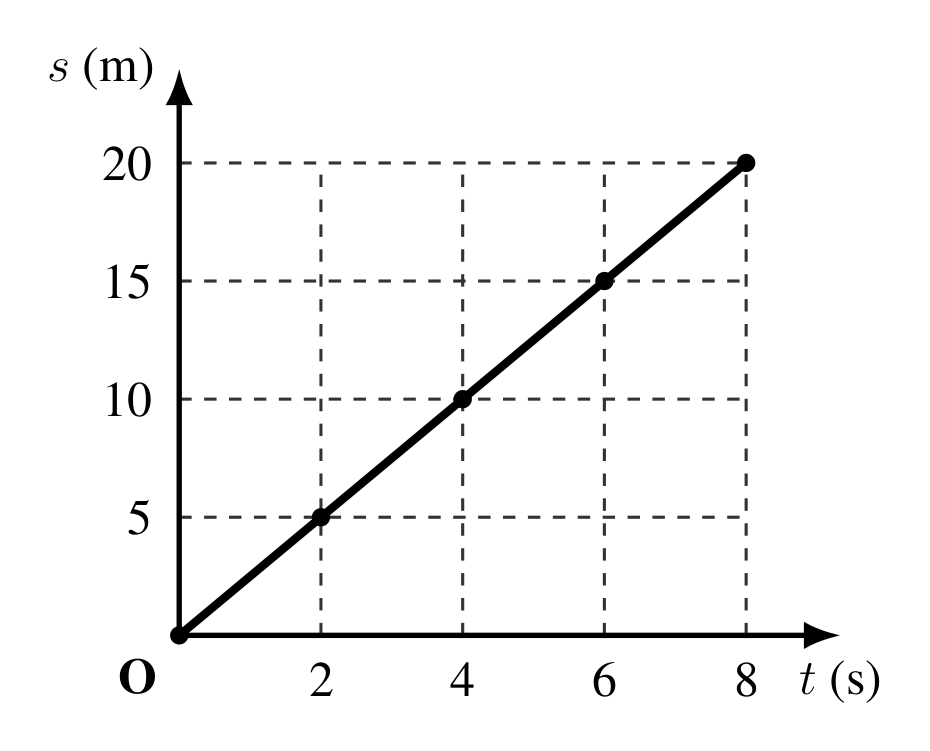
\includegraphics[width=6.5cm]{images_khtn7/do_thi_cau5.png}
\end{center}

\begin{enumerate}[label=\alph*.,leftmargin=1.5cm,itemsep=1pt]
  \item Xác định quãng đường đi được của vật sau $8\text{ s}$ kể từ lúc xuất phát.
  \item Sau bao lâu kể từ lúc xuất phát vật đi hết quãng đường $15\text{ m}$?
  \item Sau $2\text{ s}$ kể từ lúc xuất phát vật đi hết quãng đường là bao nhiêu?
  \item Từ đồ thị, hãy xác định tốc độ của vật.
\end{enumerate}

\begin{quote}\small
{\color{myBlue}\textbf{► Lời giải chi tiết:}}
\begin{itemize}[leftmargin=*,itemsep=1pt,topsep=1pt]
  \item \textbf{a.} Từ điểm $t = 8\text{ s}$ trên trục hoành, dóng thẳng đứng lên gặp đồ thị rồi dóng ngang sang trục tung, ta được: $s = \mathbf{20\text{ m}}$.
  \item \textbf{b.} Từ điểm $s = 15\text{ m}$ trên trục tung, dóng sang phải gặp đồ thị rồi dóng thẳng xuống trục hoành, ta được: $t = \mathbf{6\text{ s}}$.
  \item \textbf{c.} Từ điểm $t = 2\text{ s}$ trên trục hoành, dóng lên gặp đồ thị rồi dóng sang trục tung, ta được: $s = \mathbf{5\text{ m}}$.
  \item \textbf{d.} Vì đồ thị là đoạn thẳng qua gốc tọa độ nên vật chuyển động thẳng đều. Tốc độ của vật là: $v = \dfrac{s}{t} = \dfrac{20}{8} = \mathbf{2{,}5\text{ m/s}}$ (hay $9\text{ km/h}$).
\end{itemize}
\end{quote}

\textbf{6.} Bảng dưới đây ghi lại quãng đường đi được theo thời gian của một người đi bộ:

\begin{center}
\begin{tabular}{|l|c|c|c|c|c|c|}
\hline
\textbf{Thời gian (s)} & 0 & 10 & 20 & 30 & 40 & 50 \\ \hline
\textbf{Quãng đường (m)} & 0 & 14 & 28 & 42 & 56 & 70 \\ \hline
\end{tabular}
\end{center}

\begin{enumerate}[label=\alph*.,leftmargin=1.5cm,itemsep=1pt]
  \item Dựa vào số liệu trong bảng, hãy vẽ đồ thị quãng đường - thời gian của người đi bộ.
  \item Từ đồ thị, xác định tốc độ đi bộ của người đó.
\end{enumerate}

\begin{quote}\small
{\color{myBlue}\textbf{► Lời giải chi tiết:}}
\begin{itemize}[leftmargin=*,itemsep=1pt,topsep=1pt]
  \item \textbf{a. Đồ thị quãng đường - thời gian:}
    \begin{center}
    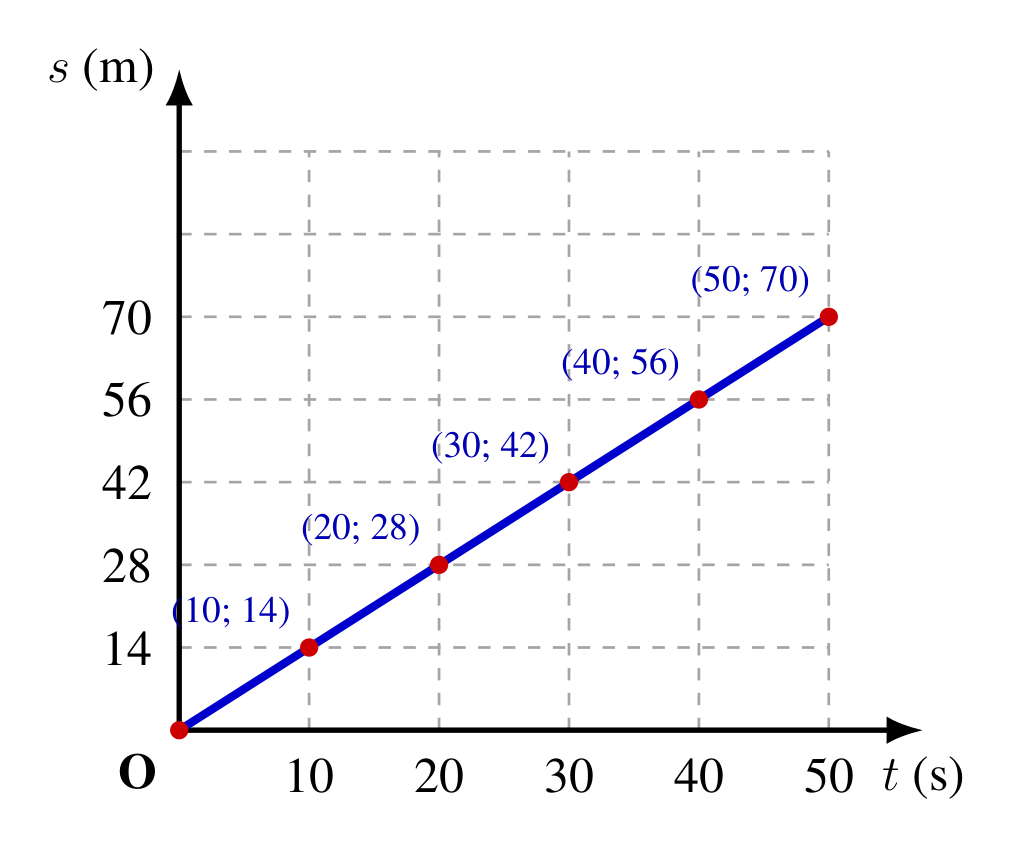
\includegraphics[width=6.5cm]{images_khtn7/do_thi_cau6.png}
    \end{center}
    Vẽ hệ trục $sOt$, xác định các điểm $O(0;0), A(10;14), B(20;28), C(30;42), D(40;56), E(50;70)$ rồi nối các điểm bằng đường thẳng xiên góc.
  \item \textbf{b. Tốc độ đi bộ của người đó:}
    Người đó chuyển động đều vì sau những khoảng thời gian 10 s bằng nhau đều đi được 14 m.
    $$v = \dfrac{s}{t} = \dfrac{14}{10} = \mathbf{1{,}4\text{ m/s}} = 1{,}4 \times 3{,}6 = \mathbf{5{,}04\text{ km/h}}.$$
\end{itemize}
\end{quote}

\vspace{6pt}
{\color{myGreen}\large\bfseries II. KHTN (HÓA HỌC)}

\vspace{3pt}
{\color{mySub}\textbf{A. Lý thuyết:}}

\textbf{1.} Bài 1: Phần II: Một số kĩ năng tiến trình học tập môn khoa học tự nhiên: quan sát, phân loại, liên kết, đo, dự báo.

\begin{quote}\small
{\color{myBlue}\textbf{► Lời giải chi tiết:}}
\begin{itemize}[leftmargin=*,itemsep=1pt,topsep=1pt]
  \item \textbf{Kĩ năng quan sát:} Thu nhận thông tin về đối tượng, hiện tượng bằng các giác quan hoặc dụng cụ hỗ trợ (kính lúp, kính hiển vi...).
  \item \textbf{Kĩ năng phân loại:} Nhóm các đối tượng, sự vật có đặc điểm tương đồng vào các nhóm theo tiêu chí xác định.
  \item \textbf{Kĩ năng liên kết:} Kết nối tri thức đã có với dữ liệu mới để giải thích nguyên nhân và tìm ra quy luật bản chất.
  \item \textbf{Kĩ năng đo:} Dùng các dụng cụ đo thích hợp (cân, thước, nhiệt kế...) để định lượng số liệu chính xác.
  \item \textbf{Kĩ năng dự báo:} Đưa ra phán đoán có cơ sở khoa học về kết quả hoặc xu hướng của hiện tượng.
\end{itemize}
\end{quote}

\textbf{2.} Chương I. Nguyên tử. Sơ lược về bảng tuần hoàn các nguyên tố hóa học.
\begin{itemize}[leftmargin=*,itemsep=1pt]
  \item Trình bày được mô hình nguyên tử của Rutherford - Bohr: mô hình sắp xếp electron trong các lớp của vỏ nguyên tử, cấu tạo nguyên tử (hạt nhân và lớp vỏ nguyên tử).
  \item Nêu được khối lượng của một nguyên tử theo đơn vị quốc tế amu (đơn vị khối lượng nguyên tử), khối lượng amu các hạt proton, neutron, electron, từ đó tính khối lượng nguyên tử.
\end{itemize}

\begin{quote}\small
{\color{myBlue}\textbf{► Lời giải chi tiết:}}
\begin{itemize}[leftmargin=*,itemsep=1pt,topsep=1pt]
  \item \textbf{Mô hình Rutherford - Bohr:}
    \begin{itemize}
      \item \textit{Cấu tạo nguyên tử:} Gồm hạt nhân mang điện dương ở tâm (chứa proton mang điện $+1$ và neutron không mang điện) và lớp vỏ gồm các electron mang điện âm ($-1$) quay xung quanh. Do trung hòa về điện nên: $\text{Số } p = \text{Số } e$.
      \item \textit{Sắp xếp electron:} Phân bố thành từng lớp từ trong ra ngoài: Lớp 1 tối đa $2\text{ e}$; Lớp 2 tối đa $8\text{ e}$; Lớp 3 tối đa $8\text{ e}$.
    \end{itemize}
  \item \textbf{Khối lượng nguyên tử theo amu:}
    \begin{itemize}
      \item $1\text{ amu} \approx 1{,}6605 \times 10^{-24}\text{ g}$.
      \item $m_p \approx 1\text{ amu}$, $m_n \approx 1\text{ amu}$, $m_e \approx 0{,}00055\text{ amu}$ (rất nhỏ có thể bỏ qua).
      \item Khối lượng nguyên tử tập trung hầu hết ở hạt nhân: $m_{\text{nguyên tử}} \approx m_p + m_n \approx (\text{Số } p + \text{Số } n)\text{ amu}$.
    \end{itemize}
\end{itemize}
\end{quote}

\vspace{4pt}
{\color{mySub}\textbf{B. Một số bài tập vận dụng:}}

\textbf{1.} Quan sát hình 2.1 sgk và cho biết các thành phần cấu tạo của nguyên tử.

\begin{quote}\small
{\color{myBlue}\textbf{► Lời giải chi tiết:}}
Nguyên tử gồm 2 thành phần chính:
\begin{itemize}[leftmargin=*,itemsep=1pt]
  \item \textbf{Hạt nhân:} Nằm ở trung tâm nguyên tử, mang điện tích dương, gồm proton ($p$) mang điện dương và neutron ($n$) không mang điện.
  \item \textbf{Lớp vỏ nguyên tử:} Bao quanh hạt nhân, gồm các electron ($e$) mang điện tích âm chuyển động quanh hạt nhân.
\end{itemize}
\end{quote}

\textbf{2.} Quan sát hình 2.2 sgk áp dụng mô hình nguyên tử của Bo, mô tả cấu tạo của nguyên tử hydrogen, và nguyên tử carbon.

\begin{quote}\small
{\color{myBlue}\textbf{► Lời giải chi tiết:}}
\begin{itemize}[leftmargin=*,itemsep=1pt]
  \item \textbf{Nguyên tử Hydrogen (H):} Hạt nhân chứa 1 proton ($+1$); lớp vỏ có 1 electron ($-1$) trên 1 lớp electron; khối lượng $\approx 1\text{ amu}$.
  \item \textbf{Nguyên tử Carbon (C):} Hạt nhân chứa 6 proton ($+6$) và 6 neutron ($0$); lớp vỏ có 6 electron trên 2 lớp (lớp 1 có $2\text{ e}$, lớp 2 có $4\text{ e}$); khối lượng $\approx 12\text{ amu}$.
\end{itemize}
\end{quote}

\textbf{3.} Khi tìm hiểu về mô hình nguyên tử carbon theo Rutherford – Bohr, người ta xác định được hạt nhân nguyên tử chứa 6 proton, 6 neutron và vỏ nguyên tử chứa 6 electron.
\begin{enumerate}[label=\alph*.,leftmargin=1.5cm,itemsep=1pt]
  \item Ở lớp vỏ nguyên tử carbon, 6 electron được phân bố thành 2 lớp. Vẽ mô hình cấu tạo nguyên tử Carbon.
  \item Biết rằng khối lượng nguyên tử tập trung chủ yếu ở hạt nhân và coi khối lượng mỗi proton và neutron xấp xỉ 1 amu. Tính khối lượng của nguyên tử carbon bao nhiêu amu?
\end{enumerate}

\begin{quote}\small
{\color{myBlue}\textbf{► Lời giải chi tiết:}}
\begin{itemize}[leftmargin=*,itemsep=1pt]
  \item \textbf{a. Mô hình cấu tạo nguyên tử Carbon:}
    \begin{center}
    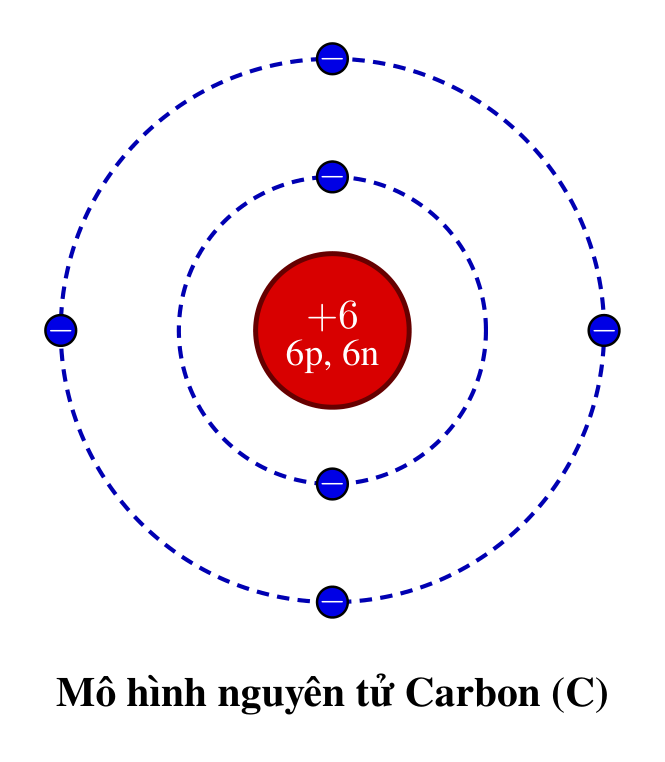
\includegraphics[width=4.5cm]{images_khtn7/mo_hinh_carbon.png}
    \end{center}
    Phân bố electron: Lớp 1 (trong cùng) có $2\text{ e}$, lớp 2 (ngoài cùng) có $4\text{ e}$.
  \item \textbf{b. Khối lượng nguyên tử Carbon:}
    $m_C \approx m_p + m_n = (6 \times 1) + (6 \times 1) = \mathbf{12\text{ amu}}$.
\end{itemize}
\end{quote}

\textbf{4.} Khi tìm hiểu cấu tạo nguyên tử nhôm (Aluminium) theo mô hình Rutherford – Bohr, học sinh xác định được trong hạt nhân nguyên tử này có 13 proton.
\begin{enumerate}[label=\alph*.,leftmargin=1.5cm,itemsep=1pt]
  \item Em hãy vẽ sơ đồ mô hình nguyên tử nhôm theo Rutherford – Bohr.
  \item Biết nhôm có khối lượng nguyên tử 27 amu, khối lượng mỗi proton và neutron xấp xỉ 1 amu. Tính số hạt neutron.
\end{enumerate}

\begin{quote}\small
{\color{myBlue}\textbf{► Lời giải chi tiết:}}
\begin{itemize}[leftmargin=*,itemsep=1pt]
  \item \textbf{a. Sơ đồ mô hình nguyên tử Nhôm (Aluminium):}
    \begin{center}
    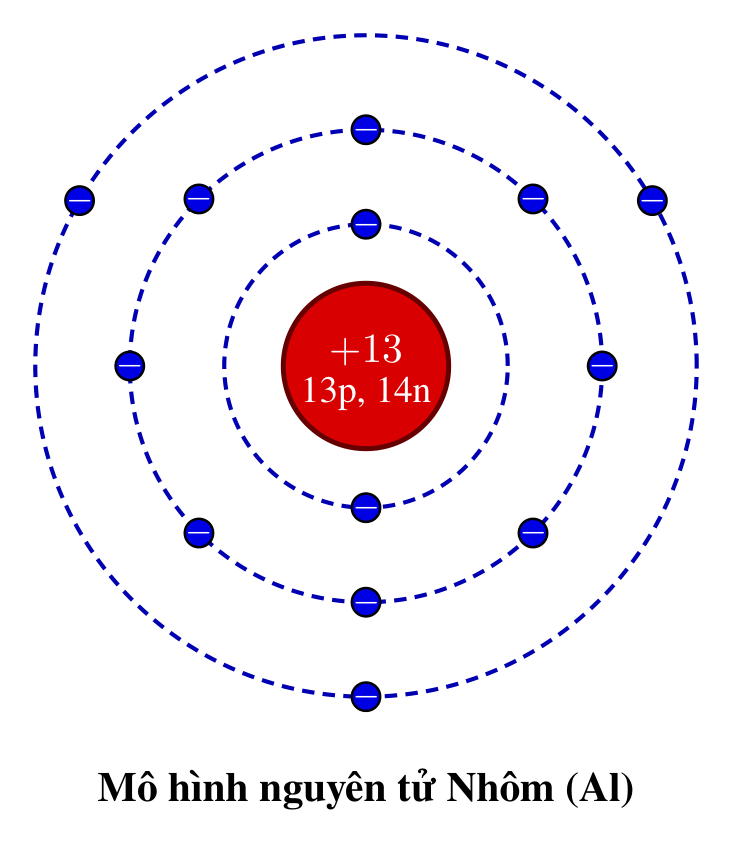
\includegraphics[width=4.8cm]{images_khtn7/mo_hinh_aluminium.png}
    \end{center}
    Số electron = Số proton = $13$. Phân bố thành 3 lớp: Lớp 1 có $2\text{ e}$, Lớp 2 có $8\text{ e}$, Lớp 3 có $3\text{ e}$.
  \item \textbf{b. Tính số hạt neutron trong nguyên tử Nhôm:}
    $$\text{Khối lượng } \approx \text{Số } p + \text{Số } n \implies \text{Số } n = 27 - 13 = \mathbf{14\text{ hạt neutron}}.$$
\end{itemize}
\end{quote}

\vspace{6pt}
{\color{myGreen}\large\bfseries III. KHTN (SINH HỌC)}

\vspace{3pt}
{\color{mySub}\textbf{A. Trắc nghiệm \& Câu hỏi ôn tập trọng tâm:}}

\textbf{1.} Khái niệm, vai trò của trao đổi chất và chuyển hóa năng lượng.

\begin{quote}\small
{\color{myBlue}\textbf{► Lời giải chi tiết:}}
\begin{itemize}[leftmargin=*,itemsep=1pt]
  \item \textbf{Khái niệm:}
    \begin{itemize}
      \item \textit{Trao đổi chất:} Quá trình cơ thể lấy các chất từ môi trường ngoài vào, biến đổi thành chất cần thiết cho cơ thể và thải chất cặn bã ra ngoài.
      \item \textit{Chuyển hóa năng lượng:} Biến đổi năng lượng từ dạng này sang dạng khác trong tế bào và cơ thể (quang năng $\to$ hóa năng, hóa năng $\to$ nhiệt năng/cơ năng).
    \end{itemize}
  \item \textbf{Vai trò:} Cung cấp nguyên liệu để xây dựng cơ thể; cung cấp năng lượng (ATP) cho mọi hoạt động sống; bài tiết chất thải duy trì cân bằng nội môi.
\end{itemize}
\end{quote}

\textbf{2.} Các yếu tố ảnh hưởng đến quang hợp như thế nào?

\begin{quote}\small
{\color{myBlue}\textbf{► Lời giải chi tiết:}}
\begin{itemize}[leftmargin=*,itemsep=1pt]
  \item \textbf{Ánh sáng:} Cung cấp năng lượng cho quang hợp; cường độ ánh sáng tăng thì quang hợp tăng đến điểm bão hòa.
  \item \textbf{Nồng độ $\text{CO}_2$:} Là nguyên liệu tổng hợp chất hữu cơ; nồng độ $\text{CO}_2$ tăng giúp tăng hiệu suất quang hợp (quá cao sẽ gây hại).
  \item \textbf{Nước:} Vừa là nguyên liệu trực tiếp, vừa điều hòa khí khổng mở để nhận $\text{CO}_2$.
  \item \textbf{Nhiệt độ:} Ảnh hưởng hoạt tính enzyme quang hợp (nhiệt độ tối ưu $25^\circ\text{C} - 35^\circ\text{C}$).
  \item \textbf{Chất khoáng:} Tham gia cấu tạo phân tử diệp lục và hệ enzyme.
\end{itemize}
\end{quote}

\textbf{3.} Các yếu tố ảnh hưởng đến hô hấp tế bào như thế nào?

\begin{quote}\small
{\color{myBlue}\textbf{► Lời giải chi tiết:}}
\begin{itemize}[leftmargin=*,itemsep=1pt]
  \item \textbf{Nước:} Môi trường và tham gia phản ứng hô hấp; độ ẩm cao làm tăng hô hấp.
  \item \textbf{Nhiệt độ:} Ảnh hưởng hoạt tính enzyme hô hấp (tối ưu $30^\circ\text{C} - 35^\circ\text{C}$); nhiệt độ thấp ức chế hô hấp, nhiệt độ quá cao làm enzyme biến tính.
  \item \textbf{Hàm lượng $\text{O}_2$:} Nguyên liệu trực tiếp oxy hóa chất hữu cơ; thiếu $\text{O}_2$ tế bào chuyển sang lên men kị khí.
  \item \textbf{Hàm lượng $\text{CO}_2$:} Là sản phẩm hô hấp; nồng độ $\text{CO}_2$ cao ($> 3\% - 5\%$) gây ức chế hô hấp tế bào.
\end{itemize}
\end{quote}

\textbf{4.} Đặc điểm cấu tạo của lá phù hợp với chức năng quang hợp.

\begin{quote}\small
{\color{myBlue}\textbf{► Lời giải chi tiết:}}
\begin{itemize}[leftmargin=*,itemsep=1pt]
  \item \textbf{Hình thái bên ngoài:} Phiến lá rộng, mỏng thu nhận nhiều ánh sáng; lá mọc so le tránh che khuất nhau; hệ gân lá vận chuyển nước và chất hữu cơ.
  \item \textbf{Cấu tạo bên trong:} Biểu bì có lớp cutin trong suốt và nhiều \textit{khí khổng} đóng mở trao đổi khí; lớp mô giậu chứa nhiều \textit{lục lạp (chứa diệp lục)} để quang hợp; lớp mô khuyết chứa khoảng gian bào trao đổi khí.
\end{itemize}
\end{quote}

\textbf{5.} Khái niệm, phương trình tổng quát của quang hợp, hô hấp tế bào.

\begin{quote}\small
{\color{myBlue}\textbf{► Lời giải chi tiết:}}
\begin{itemize}[leftmargin=*,itemsep=1pt]
  \item \textbf{Quang hợp:}
    \begin{itemize}
      \item Khái niệm: Lục lạp hấp thụ ánh sáng mặt trời tổng hợp glucose từ $\text{CO}_2$ và $\text{H}_2\text{O}$, giải phóng $\text{O}_2$.
      \item Phương trình: $\text{Nước} + \text{Carbon dioxide} \xrightarrow[\text{Diệp lục}]{\text{Ánh sáng}} \text{Glucose} + \text{Oxygen}$
      \item $(6\text{H}_2\text{O} + 6\text{CO}_2 \xrightarrow[\text{Diệp lục}]{\text{Ánh sáng}} \text{C}_6\text{H}_{12}\text{O}_6 + 6\text{O}_2\uparrow)$
    \end{itemize}
  \item \textbf{Hô hấp tế bào:}
    \begin{itemize}
      \item Khái niệm: Phân giải hợp chất hữu cơ (glucose) thành $\text{CO}_2$ và $\text{H}_2\text{O}$, giải phóng năng lượng ATP và nhiệt.
      \item Phương trình: $\text{Glucose} + \text{Oxygen} \xrightarrow{\text{Enzyme}} \text{Carbon dioxide} + \text{Nước} + \text{Năng lượng (ATP + Nhiệt)}$
      \item $(\text{C}_6\text{H}_{12}\text{O}_6 + 6\text{O}_2 \xrightarrow{\text{Enzyme}} 6\text{CO}_2 + 6\text{H}_2\text{O} + \text{ATP + Nhiệt})$
    \end{itemize}
\end{itemize}
\end{quote}

\textbf{6.} Mối quan hệ giữa tổng hợp và phân giải chất hữu cơ ở tế bào.

\begin{quote}\small
{\color{myBlue}\textbf{► Lời giải chi tiết:}}
Là hai mặt đối lập nhưng thống nhất mật thiết:
\begin{itemize}[leftmargin=*,itemsep=1pt]
  \item \textit{Đối lập:} Tổng hợp tích lũy chất hữu cơ và hóa năng; phân giải giải phóng chất vô cơ và năng lượng ATP.
  \item \textit{Thống nhất:} Tổng hợp tạo ra nguyên liệu (glucose, protein...) cho phân giải; ngược lại phân giải cung cấp năng lượng ATP và chất trung gian cho tổng hợp. Nếu một quá trình dừng lại, sinh vật sẽ chết.
\end{itemize}
\end{quote}

\textbf{7.} Ý nghĩa của việc trồng và bảo vệ cây xanh.

\begin{quote}\small
{\color{myBlue}\textbf{► Lời giải chi tiết:}}
\begin{itemize}[leftmargin=*,itemsep=1pt]
  \item Điều hòa khí hậu, cân bằng hàm lượng $\text{CO}_2$ và $\text{O}_2$ trong khí quyển.
  \item Lọc bụi bẩn, hấp thụ khí độc, giảm ô nhiễm tiếng ồn và làm mát môi trường sống.
  \item Chống xói mòn đất, giữ nước ngầm, giảm thiểu nguy cơ lũ lụt, hạn hán.
  \item Cung cấp thức ăn, nơi cư trú cho sinh vật; cung cấp gỗ, thực phẩm, dược liệu cho con người.
  \item Tạo cảnh quan thiên nhiên trong lành, xanh sạch đẹp.
\end{itemize}
\end{quote}

\vspace{4pt}
{\color{mySub}\textbf{B. Tự luận:}}

\textbf{Vận dụng hô hấp tế bào vào thực tiễn:} Giải thích vì sao rau củ quả thường được bảo quản trong ngăn mát tủ lạnh. Vì sao một số loại thực phẩm bảo quản quá lâu thì bị giảm chất lượng\dots

\begin{quote}\small
{\color{myBlue}\textbf{► Lời giải chi tiết:}}
\begin{enumerate}[leftmargin=*,itemsep=2pt]
  \item \textbf{Vì sao rau củ quả bảo quản trong ngăn mát tủ lạnh:}
    \begin{itemize}
      \item Rau củ quả sau thu hoạch vẫn là tế bào sống, liên tục diễn ra hô hấp tiêu hao chất hữu cơ, nước và sinh nhiệt.
      \item Ngăn mát tủ lạnh duy trì $1^\circ\text{C} - 4^\circ\text{C}$. Ở nhiệt độ thấp này, hoạt tính \textbf{enzyme hô hấp bị ức chế mạnh}, cường độ hô hấp giảm tối thiểu, kìm hãm vi sinh vật và nấm mốc phát triển, làm chậm thoát hơi nước, giúp rau củ giữ nguyên độ tươi ngon và dinh dưỡng lâu hơn.
    \end{itemize}
  \item \textbf{Vì sao bảo quản quá lâu thì bị giảm chất lượng:}
    \begin{itemize}
      \item Quá trình hô hấp vẫn diễn ra chậm chạp liên tục, làm tiêu hao dần các chất dinh dưỡng (đường, vitamin...), làm củ bị xốp, nhạt nhẽo.
      \item Mất nước vi mô khiến rau củ bị mềm nhũn, mất độ giòn; một số củ mọc mầm (khoai tây sinh độc tố solanine).
      \item Vi sinh vật kị khí hoặc nấm mốc chịu lạnh sau thời gian dài vẫn thích nghi và phát triển, làm biến tính chất lượng, gây mùi chua, ôi thiu.
    \end{itemize}
\end{enumerate}
\end{quote}

\end{document}
